\documentclass[a4paper,11pt]{report}
\usepackage[latin1]{inputenc}
\usepackage[english]{babel}
\usepackage{graphicx} 
\usepackage{pdfpages}
\usepackage{fancyvrb}
\usepackage{pdflscape}
\usepackage{fancyhdr}
\pagestyle{fancy}

\bibliographystyle{unsrt}

\fancyhead[CO,CE]{---MidTerm Report--}
\fancyhead[RO, LE] {\thepage}
\renewcommand{\headrulewidth}{0.4pt}
\renewcommand{\footrulewidth}{0.4pt}


\begin{document}

\begin{titlepage}
\begin{center}

\includegraphics[width=5cm]{EURECOM_logo_quadri}
\\[3cm]
\textbf{\Huge{MidTerm Report}}
\\[4cm]
\textbf{\textsc{\LARGE{Publishing and Consuming Government Linked Data on the Semantic Web}}}
\\[0.5cm]
\LARGE{Ghislain Auguste Atemezing}
\\[0.5cm]
\small{EURECOM-Multimedia Communications}
\\
\large{Institut Mines-T\'{e}l\'{e}com}
\\
\large{December 19th, 2012}
\\[5cm]
\columnsep3cm
\begin{tabular}{p{8cm} p{8.5cm}}
\small{\textbf{Supervisor:}\newline
Rapha\"el Troncy} 
&
\small{\textbf{EURECOM\newline Multimedia Department}}
\end{tabular}
\end{center}
\end{titlepage}

 \tableofcontents

\chapter*{Abstract}
\addcontentsline{toc}{chapter}{Abstract}

The need for geolocation is crucial for many applications for both human and software agents. More and more data is opened and interlinked using Linked Data principles, and it is worth modeling geographic data efficiently by reusing as much as possible from existing ontologies or vocabularies that describe both the geospatial features and their shapes. Our aim is to contribute to the actual efforts in representing geographic objects with attributes such as location, points of interest (POI), and addresses in the web of data, with a special focus on the French territory.
As we publish data in RDF graphs, we are also aware of making them useful for the users. For that, we not only develop innovative applications to show up the value of data visualizations, but rather go beyond it. The challenge is to detect patterns to automatically develop an application using adequate visualization widgets in an affordable effort.  


%###Research problems####

\chapter{Research Problems}

\section{Introduction}
The Web is currently in a transition phase. After having been accessible on personal computers, it is now 
quickly moving to more and more ubiquity and entering in every part and moment of our lives. New 
devices and new ways to use them are being created. The ubiquity of the Web also creates an unseen 
abundance of information. Data is flowing onto the Web, created by users, generated by sensors, and 
stored in ever growing data farms. Geographic data is widely present on the web as they are used for location 
of Point of Interest. At the same time, many organizations are moving from legacy data stored in their databases
to structured data on the web. Structured data is already present in the many databases, metadata attached to medias, and in the millions of spreadsheets created everyday across the world. 

However, the recent emergence of linked data radically changes the way structured data is being considered. By giving standard formats for the publication and interconnection of structured data, linked data transforms the Web into a giant database. While making data available on the web, we need to build meaningful applications to show the value of all the huge data so that users could easily explore it, and derive new insights for it. As many information visualization tools are already present in InfoVis community\footnote{http://en.wikipedia.org/wiki/Information\_visualization}, their easy adoption and usage for displaying structured data raise new challenges. Those challenges are twofolds:
\begin{itemize}
\item How to characterize semantic web applications in terms of tools, widgets that can easily visualize RDF datasets.
\item Mining heterogeneous structured data to derive patterns for automatically recommend the adequate visualization tool to help users building innovative applications in an affordable time.
\end{itemize}


%####section contributions######

\section{Contributions}
   
The present report aims at giving a summary of the activities we have been accomplishing
during the first year of our thesis entitled: \textbf{``Publishing and Consuming Government Linked Data on the Semantic Web''}. Our main purpose was to first understand the problematic by an extensive state-of-the-art in : 
\begin{itemize}
\item (i)- Geographic Information on the Web of data, and 
\item (ii) visualization tools for building innovative applications consuming structured data. 
\end{itemize}



\chapter{Modeling Geographic Information in LOD} \label{model}

The need for geolocation is crucial for many applications for both human and software agents. More and more data is opened and interlinked using Linked Data principles, and it is worth modeling geographic data efficiently by reusing as much as possible from existing ontologies or vocabularies that describe both the geospatial features and their shapes. In the first part of our work, we survey different modeling approaches used by the Geographic Information System (GIS) and the Linked Open Data (LOD) communities. Our aim is to contribute to the actual efforts in representing geographic objects with attributes such as location, points of interest (POI), and addresses on the web of data. We focus on the French territory and we provide examples of representative vocabularies that can be used for describing geographic objects. We propose some alignments between various vocabularies (DBpedia, GeoNames, Schema.org, LinkedGeoData, Foursquare, etc.) in order to enable interoperability while interconnecting French geodata with other datasets. In France, there is  currently a joint effort to publish geographic information in RDF  and interlink them with relevant datasets. GeOnto is an ontology describing geospatial features for the French territory. We have proposed to align GeOnto with other popular vocabularies in the geospatial domain, using Silk for schema mapping and we have evaluated the results. We studied how to extend the model to take into account efficient modeling for complex geometries. By doing so, tackle the complex geometry representation issues in the Web of Data, describing the state of implementations of geo-spatial functions in triple stores and comparing them to the new GeoSPARQL standard.  We finally made some recommendations and advocate for the reuse of the NeoGeo ontology within GeOnto to better address the IGN requirements.
This work has lead to two publications [2,4]

\chapter {Visualization Tools in Linked Government Data} \label{visu}
We first review the numerous applications that have been developed on top of datasets that have been opened by governments (UK, USA, France) and local authorities. We have then derived and proposed height use cases  that can be developed to consume data from the different main data providers in France: INSEE, DILA, IGN, FING, etc. We mention that the most interesting UCs are the ones which show the added value of having interconnected datasets. These UCs,  developed and deployed, can be useful to show the benefits of Linked Data in a variety of domains such as Education, Tourism, Cultural Heritage, Civil administrations, Judicial Court, Medicine, etc. As a good starting point, we have developed an application\footnote{http://www.eurecom.fr/~atemezin/DemoElection/} for the first round of the French election reusing five different datasets, as Figure \ref{sampleModel} shows the data model used for the design of the application. Moreover, we observed that many successful applications that have been developed visualize structured data around the geographical, time and concepts dimensions. Futhermore, we analyse some requirements expected from the users and actors/providers of Open Data in France. 

\begin{landscape}
\begin{figure}[!htbp]
  \begin{center}
    %\leavevmode
    \ifpdf
      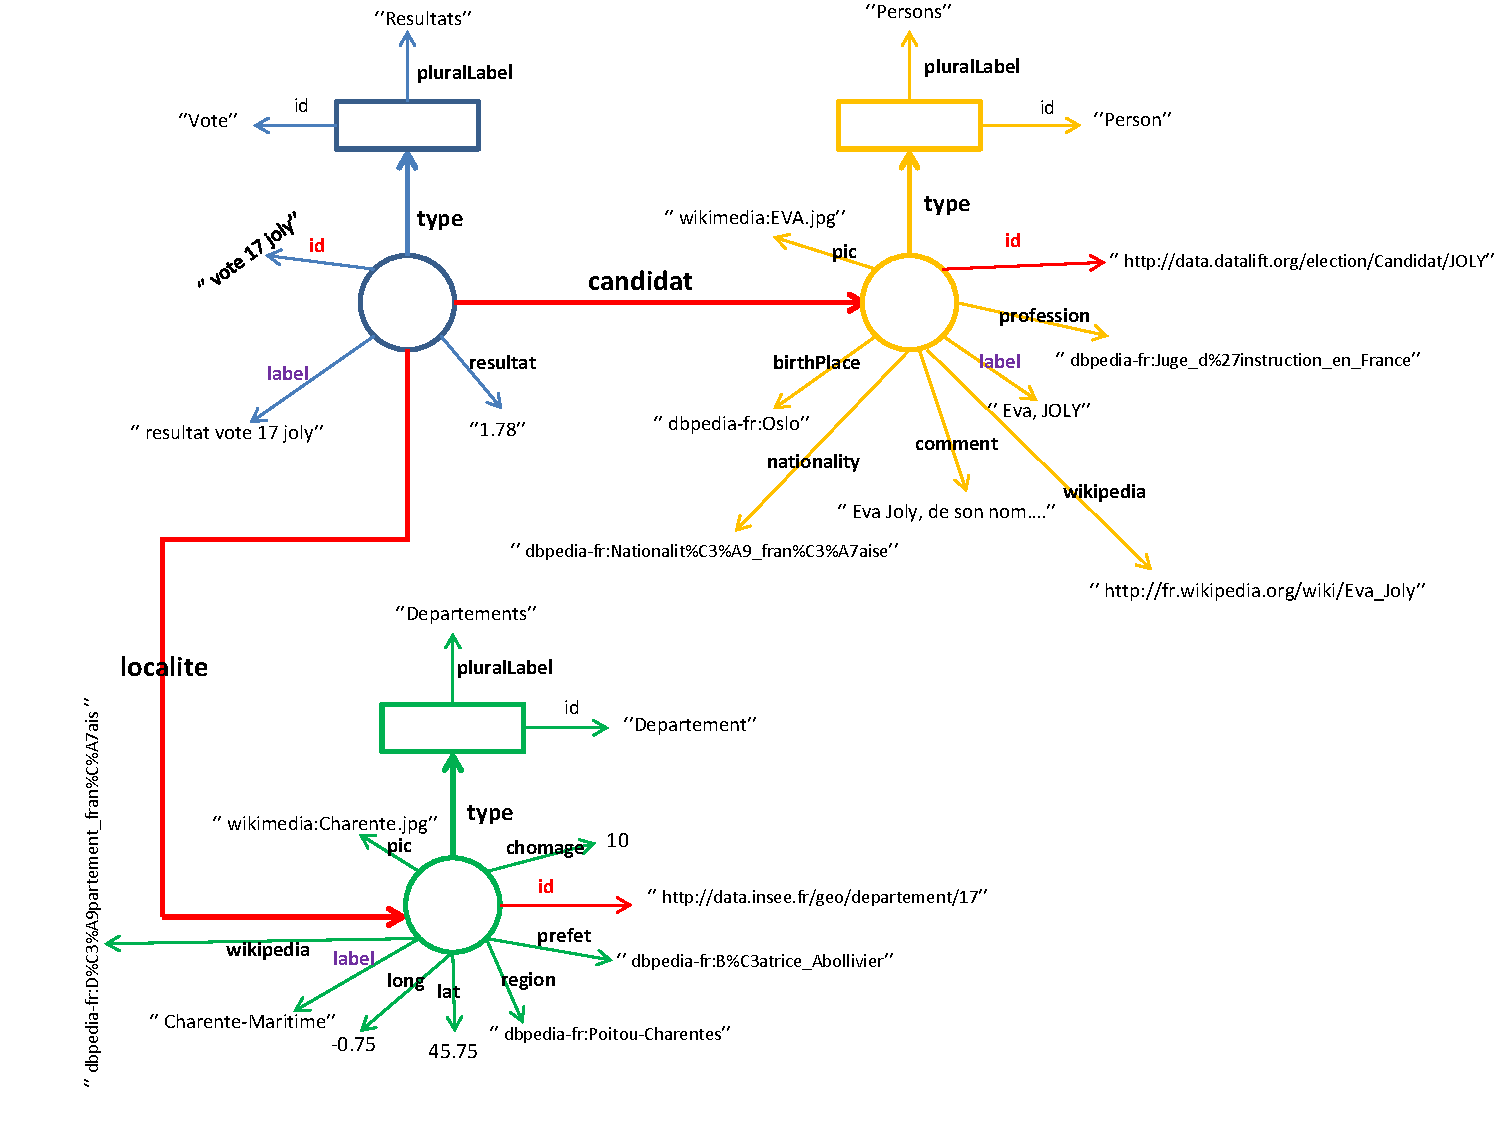
\includegraphics[height=5in]{model_EvaJoly_data}
    \else
      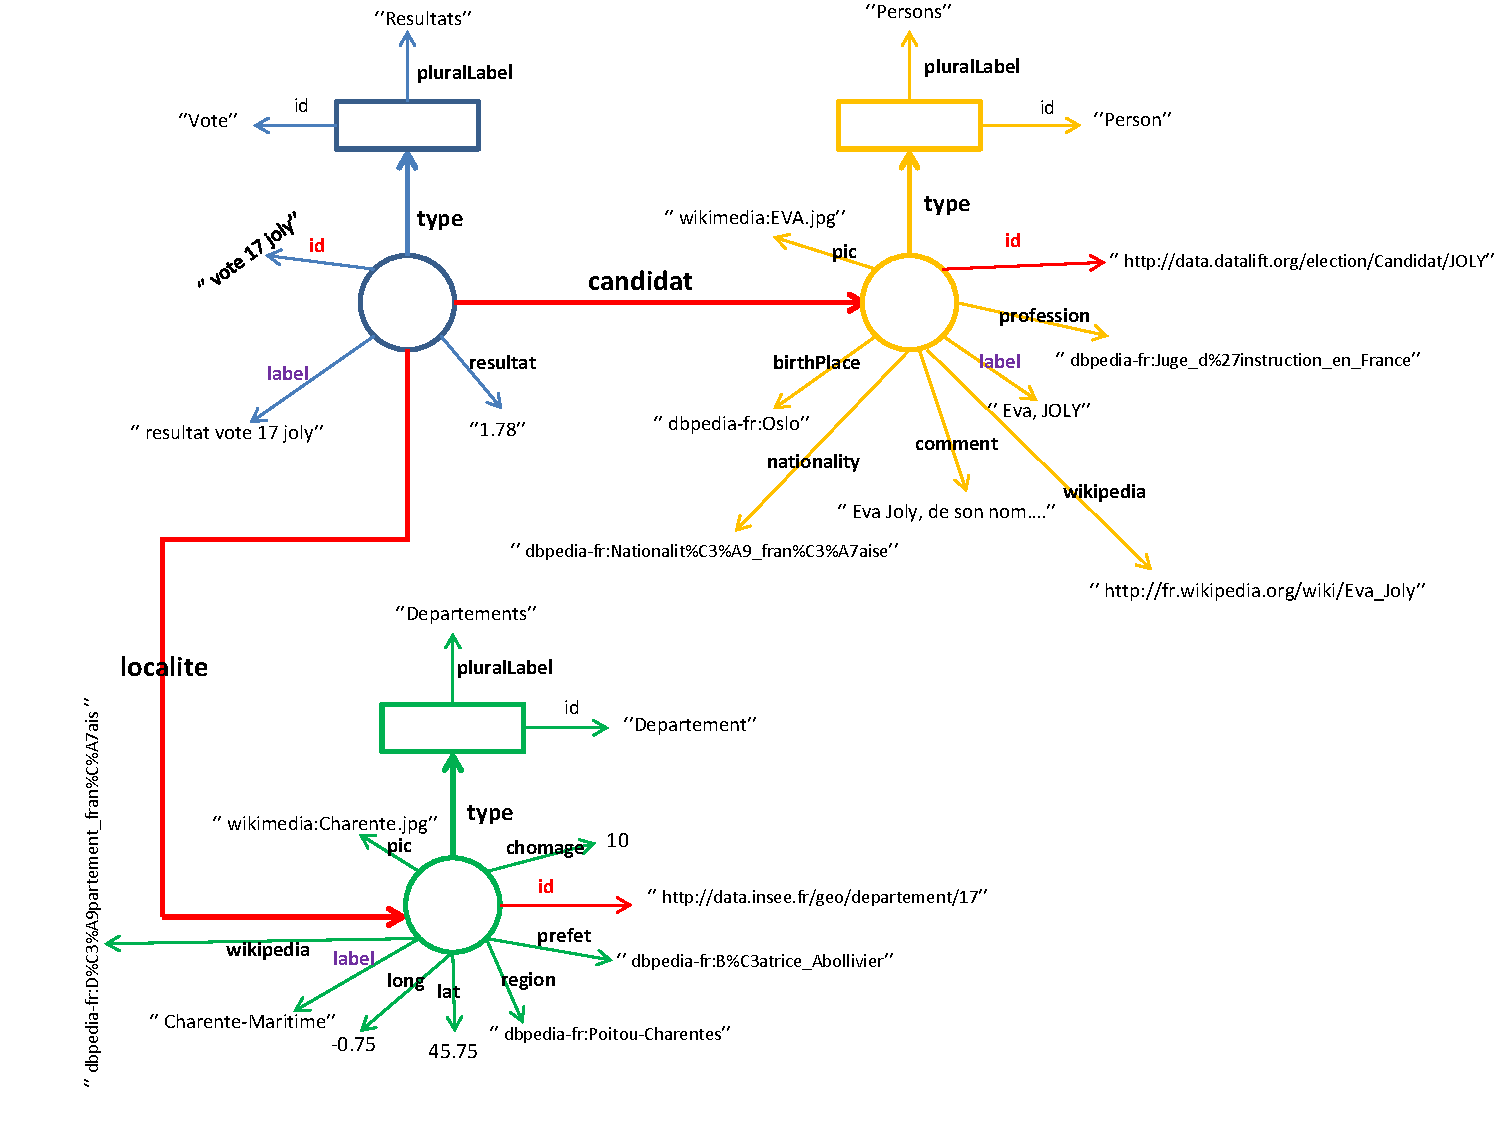
\includegraphics[bb = 92 86 545 742, height=6in]{model_EvaJoly_data}
    \fi
    \caption{Exhibit Data model of the score obtained by candidate Eva Joly in Charente-Maritime, linked with knowledge from DBpedia, INSEE and Wikipedia. }
    \label{sampleModel}
  \end{center}
\end{figure}

\end{landscape}

Regarding tools used for visualization, we have divided them in two categories, providing for each of them relevant examples: (i)-tools that operate over RDF data, (ii) and tools that operate over other structured format. We then provide some basic criteria for assessing a given visualization tool, with some weight attached to each of the criterion. 



%#####Future work###

\chapter*{Conclusions and Future work}
Regarding the geodata modeling, our future work includes the conversion and publication of a large RDF dataset of geographic information of the French territory together with alignments with other datasets at the instance level. At the same time, we plan to publish with IGN a new version of an adequate ontology for describing features and geometry according some best practices we are contributing to elaborate. Furthermore, some alignments with the new OGC standard GeoSPARQL will be performed and evaluated.
Regarding the visualization tools, some further studies should be made for mobile applications, as they are not considered in this current study. We plan also to develop a small vocabulary that could be used to describe OpenData applications. At the same time, we will develop two more applications using different datasets for detecting patterns for visualizing RDF data. For this challenge, we will need to study the underlying data (list of properties, number of triples, categories, etc.), the ontologies used, the templates or libraries for visualizations (Exhibit, GeoAPI, LDA, Sparkl, d3.js,etc) and finally the effort for a user to build the application.


%\cleardoublepage
\addcontentsline{toc}{chapter}{Bibliography}
\bibliography{biblio}

%\appendix
%\cleardoublepage
\addcontentsline{toc}{chapter}{Annexes}

\appendix
\chapter{Publications}
\section*{Journal}
\begin{itemize}
\item [1]- Su\'{a}rez-Figueroa, Mari Carmen; Atemezing, Ghislain Auguste; Corcho, Oscar : \textbf{The landscape of 
multimedia ontologies in the last decade} in  Multimedia Tools and Applications, Vol 55, Number 3, December 2011.
\end{itemize}


\section*{Conference}
\begin{itemize}
\item [2]- Atemezing, Ghislain; Troncy, Rapha\"{e}l: \textbf{Comparing vocabularies for representing geographical features and their geometry} in ISWC 2012, 11th International Semantic Web Conference, Terra Cognita, Boston, USA, November 11-15, 2012
\item [3]- Scharffe, Fran\c cois; Atemezing, Ghislain; Troncy, Rapha\"{e}l; Gandon, Fabien; Villata, Serena; Bucher, B\'{e}n\'{e}dicte; Hamdi, Fay\c cal; Bihanic, Laurent; K\'{e}p\'{e}klian, Gabriel; Cotton, Franck; Euzenat, J\'{e}r\^{o}me; Fan, Zhengjie; Vandenbussche, Pierre-Yves; Vatant, Bernard: \textbf{Enabling linked-data publication with the datalift platform} in
AAAI 2012, 26th Conference on Artificial Intelligence, W10:Semantic Cities, July 22-26, 2012, Toronto, Canada.
\item [4]- Atemezing, Ghislain; Troncy, Rapha\"{e}l : \textbf{Vers une meilleure interop\'{e}rabilit\'{e} des donn\'{e}es g\'{e}ographiques fran\c caises sur le Web de donn\'{e}es} in IC 2012, 23\'{e}mes Journ\'{e}es Francophones d'Ing\'{e}nierie des Connaissances, June 25-29, 2012, Paris, France.
\item [5]- Khrouf, Houda; Atemezing, Ghislain; Rizzo, Giuseppe; Troncy, Rapha\"{e}l; Steiner, Thomas:
\textbf{Aggregating social media for enhancing conference experiences} in RAMSS 2012, 1st International Workshop on Real-Time Analysis and Mining of Social Streams, June 4, 2012, Dublin, Ireland.
\item [6]- Khrouf, Houda; Atemezing, Ghislain; Steiner, Thomas; Rizzo, Giuseppe; Troncy, Rapha\"{e}l: 
\textbf{Confomaton: A conference enhancer with social media from the cloud} in ESWC 2012, 9th Extended Semantic Web Conference, May 27-31, 2012, Heraklion, Crete.
\end{itemize}

\section*{Talk}
\begin{itemize}
\item [7]- Bucher, Benedicte; Hart, Glen; Atemezing, Ghislain; Villazon Terrazas, Boris; Bihanic, Laurent; Roensdorf, Carsten; Hamdi, Fay\c cal; Goodwin, John; Troncy, Rapha\"{e}l; Kepeklian, Gabriel; Corcho, Oscar: 
\textbf{A practical introduction to geographical linked data : lift your data} in 
INSPIRE 2012, Infrastructure for Spatial Information in Europe, June 23-27, 2012, Istanbul, Turkey.
\end{itemize}

\section*{W3C Report}
\begin{itemize}
\item [8]- Wood, David; Atemezing, Ghislain; Hyland, Bernadette : 
\textbf{Common Glossary of Terms in Linked Data} W3C Government Linked Data Working Group, 2012.
\end{itemize}


\chapter{Project}
The work reported here has been funded in the ANR Datalift project where we develop technologies for
\begin{itemize}
\item publishing data as RDF graphs: a very simple data format, 
\item linking these data sets together, by identifying equivalent resources in other data sources,
\item describing the vocabulary used in published data through ontologies.
\item developing innovative applications on top of data sets exposed in RDF. 
\end{itemize}

\section*{Meetings}
We have been present in all the different meetings with the rest of the seven partners of the project.
Since our arrival at Eur\'{e}com, we have attended to all the General Meetings planned as follow:
\begin{itemize}
\item 03-04/09/2012, Montpellier (LIRMM)
\item 06-07/06/2012, Grenoble (INRIA-EXMO)
\item 17-18/01/2012, Paris (INSEE)
\item 29-30/09/2011, Sophia Antipolis (INRIA-WIMIX)
\end{itemize}

\section*{Deliverables}
We have produced two deliverables in the context of Datalift project: 
\begin{itemize}
\item \textbf{D6.1 : Usage scenarii for applications (v.1.1)} Authors: \texttt{Ghislain A. Atemezing (EURECOM), Charles Nepote (FING) and Rapha\"{e}l Troncy (EURECOM)}, June, 8th 2012. Reviewed by Fabien Gandon (INRIA) and Thomas Francart (Mondeca). The document describes some innovative applications consuming open data in UK, USA and France. It also shows up some relevant use cases that could be developed in the DataLift platform, considering the type of data  ``lifted'' from the data providers in the project (INSEE, IGN and DILA). It finally captures some requirements from the perspectives of the users.
\item \textbf{D6.2 : Tools for visualizing data on the Semantic Web (v.1.2)} Authors: \texttt{Ghislain A. Atemezing , Rapha\"{e}l Troncy (EURECOM)}, June, 13th 2012. Reviewed by Fabien Gandon (INRIA), Fran\c cois Scharffe (LIRMM) and Franck Cotton (INSEE). The document describes tools that operate over RDF data, revisits those tools that operate over other structured format, and finally provides some criteria to take into account when selecting a given visualization tool, with some weight attached to each of the criterion.
\end{itemize}
\end{document}
